\chapter{Memory Access Unit and Control Unit design}

In this section the Memory Access Unit is described, which gives the ARM part read and write 
access to several memories of the system. Another super-unit, the Control Unit is also described here. 
The latter keeps the state of the machine (on or off) and gives access to this register to the 
ARM part. The ARM processor can therefore switch the machine on and off as it wishes from this 
access. Before introducing these two super-units, the Avalon protocol is first described. This 
protocol allows the communications through the bridges existing between the ARM and FPGA part of
the Cyclone V.

\section{Communication between ARM and FPGA sides}

The communication between the two parts takes place via one of the priously mentionned bridges using 
the Avalon protocol described by Intel. This protocol allows 
high-speed communication. The Avalon interface has different sub-interfaces for different types 
of communication. Each type is adapted to certain applications. In this project where the protocol 
is used to communicate between master and slave devices, the Avalon MM is used. 
The Avalon MM protocol is address based which is very suitable for the needs of this project.
The read and write operations of this protocol are described right below.

\subsection{Read operation}

First, let's start by reading. The sequence diagram of the protocol for the reading operation is 
visible in Figure \ref{fig:avalon/mm_read}. In the diagram, two masters are represented but only 
the unique master case is described. In the first place, the master simply has to give
the start address to which it wants to read, the length of the burst (the number of words desired) 
as well as to switch the read and beginbursttransfer signals to high. The slave then responds 
to this with a waitrequest that goes up. The master must imperatively keep all signals except 
beginbursttransfer which returns to the low state unchanged during the waitrequest to give the 
slaves time to capture them. Once ready, the slave removes the waitrequest and informs that  
data is available by switching readdatavalid to high and sending the first word. The other words 
are then sent to the master in the order of their addresses. 

\begin{figure}[H]
  \center
  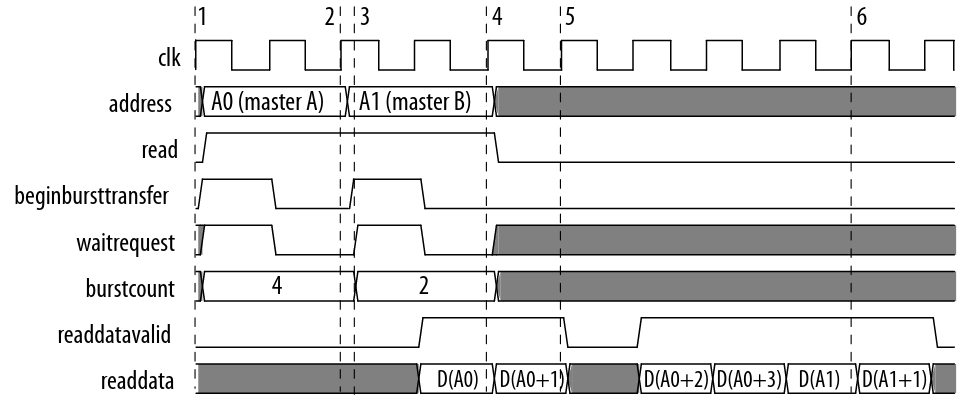
\includegraphics[width=\linewidth]{"Chapter4-MAU_CTRLU/res/avalon_mm_read.png"}
  \caption{Read operation using Avalon MM}
  \label{fig:avalon/mm_read}
\end{figure}

\subsection{Write operation}

For writing, it's even simpler. As can be seen in Figure \ref{fig:avalon/mm_write}, the beginning 
is similar to reading. The master has to provide the first address, the length of the 
burst and also to switch beginbursttransfer to high. In addition to that, the first word 
is also provided. Here again, the slave responds with a waitrequest. As soon as the waitrequest 
is switched off, the master sets the beginbusttransfer to low and send the words one after the other, 
starting at the next clock cycle. If the write signal goes down, the burst is paused and resumes 
as soon as it goes up again.

\begin{figure}[H]
  \center
  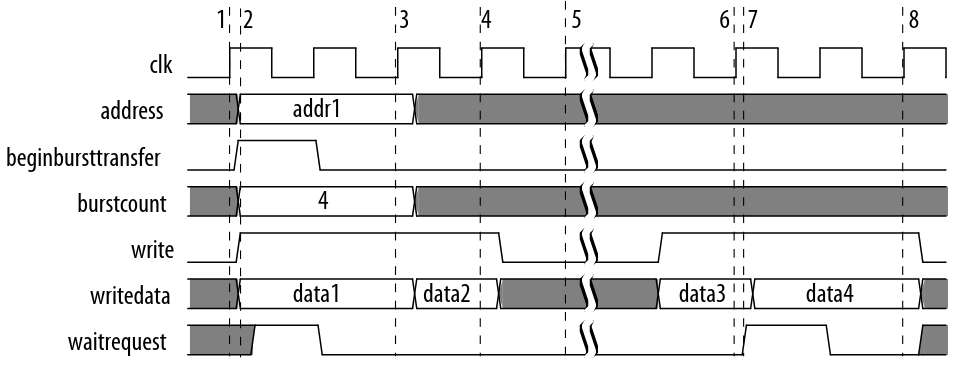
\includegraphics[width=\linewidth]{"Chapter4-MAU_CTRLU/res/avalon_mm_write.png"}
  \caption{Write operation using Avalon MM}
  \label{fig:avalon/mm_write}
\end{figure}

This protocol is not very complicated. However, it has a lot of signals and is not necessarily 
practical to use directly in user-developed slaves and masters. This is why interface modules are 
used. These modules are described in the sections where they are needed.

\section{Memory Access Unit (MAU)}

As already repeated several times the MAU allows access to several memories of the machine. In order 
to simplify the protocol in the machine, a module called Avalon to External Bus Bridge is used. This 
module manages the Avalon protocol and exposes an interface (the external bus) using a simpler 
protocol. This module is used as many times as there are memories to connect to the interconnect.
The different signals this module uses are shown in Figure \ref{fig:mau/bus_bridge}. Note that this
module has an integrated timer that is reset each time the Avalon to external bus bridge receives
an acknowledgement from the external slave. When this timer reaches 0, the request from the master 
(denoted by Avalon Switch Fabric in the Figure) is deleted.

\begin{figure}[H]
    \center
    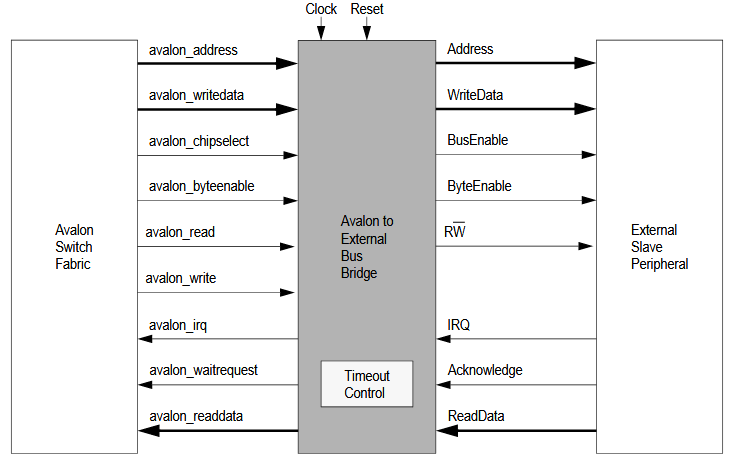
\includegraphics[scale=0.8]{"Chapter4-MAU_CTRLU/res/external_bus_bridge.PNG"}
    \caption{Avalon to external bus bridge interface and signals}
    \label{fig:mau/bus_bridge}
\end{figure}

The protocol is considered simpler because it offers an interface closer to that used by the memories 
than that of the Avalon. Indeed, the usual signals address, write data, read data and R$\overline{W}$ are 
present. Moreover, this protocol is very simple to use. Indeed, as can be seen in Figure \ref{fig:mau/bus_bridge_protocol}. The master 
places all the necessary elements on the bus and then pass the bus enable signal to high. This means 
that the slave can act. The slave then does what it has to do. Either take the data and write it to 
the address given by the master or send the requested data that is present at the address given by 
the master. Once the slave has finished its job, it switches the acknowledgement signal to high 
during a clock cycle to validate the transaction. 

\begin{figure}[H]
    \center
    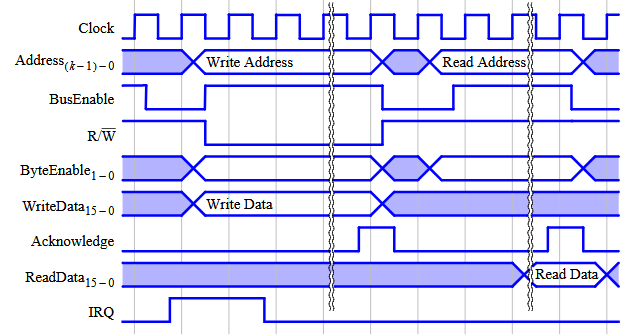
\includegraphics[scale=0.8]{"Chapter4-MAU_CTRLU/res/external_bus_timings.PNG"}
    \caption{External bus protocol timings}
    \label{fig:mau/bus_bridge_protocol}
\end{figure}

It is possible to configure the address range and the word size used by these bus. For this work, 
it is decided that the 
addressable space is 256Kbytes and that the words are on 32bits for each access except for the 
access to the GPU mask memory which is on 4Kbytes with 128bits words. Each of these accesses are 
put on the HPS-FPGA bridge, their offset is given in Table \ref{mau/bus}. These dimensions were 
chosen to make the offset easy to understand. Indeed, only the sixth number changes in the 
hexadecimal address. Moreover, this gives future users a large margin if they want to change the 
dimensions of the memories. As far as the mask memory is concerned, the address range is simply the 
size of the memory. This has been done especially to discourage any modification at this level. 
Indeed, this would lead to a large modification of the CPU which could degrade its performance or 
make it impossible to include in the design (due to lack of space on the FPGA).

\begin{table}[H]
    \centering
    \begin{tabular}{|l|c|c|c|c|}
    \hline
    \rowcolor[HTML]{DAE8FC} 
    \multicolumn{1}{|c|}{\cellcolor[HTML]{DAE8FC}\textbf{Access}} & \textbf{Base} & \textbf{End} & \textbf{Address range} & \textbf{Word size} \\ \hline
    Instruction Memory (CPU)                                      & 0x0000 0000   & 0x0003 FFFF  & 256kB             & 32                 \\ \hline
    Data Memory (CPU)                                             & 0x0010 0000   & 0x0013 FFFF  & 256kB             & 32                 \\ \hline
    Register File (CPU)                                           & 0x0020 0000   & 0x0023 FFFF  & 256kB             & 32                 \\ \hline
    I/Os (IOU)                                                    & 0x0030 0000   & 0x0033 FFFF  & 256kB             & 32                 \\ \hline
    Mask Memory (GPU)                                             & 0x0040 0000   & 0x0040 0FFF  & 4096B             & 128                \\ \hline
    \end{tabular}
    \caption{Memory bus description}
    \label{mau/bus}
\end{table}

The connections in QSys are shown in Figure \ref{fig:avalon/bus}. 
The different modules and the HPS are highlighted in 
yellow. The different Avalon slaves and the master are shown in red. It can be noticed by following 
the connection highlighted in blue that it is indeed the HPS-FPGA bridge that is used 
(h2f\_axi\_master on Qsys) and that the offsets of the slaves are indeed those previously given. The 
signals corresponding to the buses are displayed in green. Each of them is exported, that is to say 
that they can be used from the FPGA. They are the ones that are connected to the different memories.

\begin{figure}[H]
    \center
    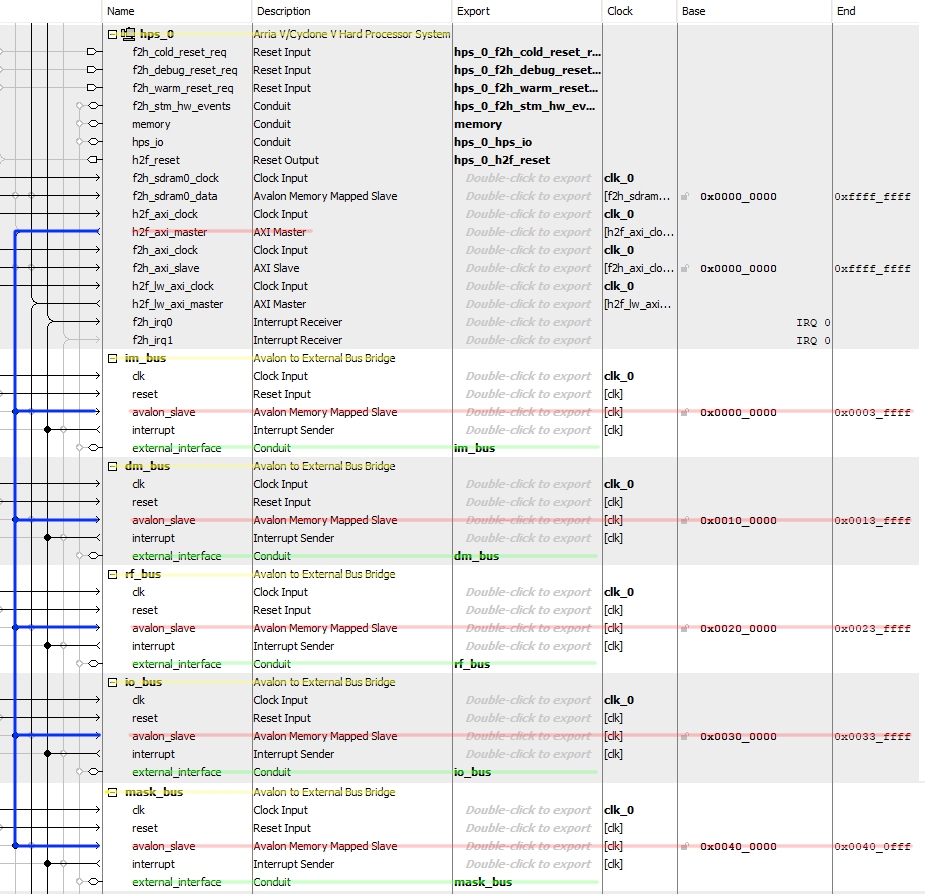
\includegraphics[width=\linewidth]{"Chapter4-MAU_CTRLU/res/qsys_mau.PNG"}
    \caption{Avalon to external bus bridges connections in Qsys}
    \label{fig:avalon/bus}
\end{figure}

Now that the description of the external bus bridge and its implementation are done, the design of 
the MAU can be considered.

\subsection{Memory Access}

In fact, the Memory Access Unit is composed of only two types of modules. The Memory Access 32, and 
the Memory Access 128 allowing both the interfacing between an external bus and a memory (having 
respectively words of 32 and 128 bits). To do this, they both implement a finite state machine. 
That of Memory Access 32 is given in Figure \ref{fig:ma_fsm}. The only difference that the 128 bits version will 
have is that the address is not multiplied by 4 in the Iddle state. 

\begin{figure}[H]
    \center
    \includegraphics[scale=0.8]{"Chapter4-MAU_CTRLU/res/mau_fsm"}
    \caption{Memory Access 32 finite state machine}
    \label{fig:ma_fsm}
\end{figure}

This state machine simply follows the protocol described earlier. It only acts when the bus is high 
and sends an acknowledge during a clock cycle once the request is executed (the finite state machine 
is reevaluated at each clock cycle). On the read side, a state seems to be useless (Read 1). This 
one is in fact very important, it gives the memory time to fetch the value present at the requested 
address. The interfaces of the memory acess are given in Figures \ref{fig:ma32} and \ref{fig:ma128}.

\begin{figure}[H]
    \center
    \includegraphics[scale=0.8]{"Chapter4-MAU_CTRLU/res/memory_access_32"}
    \caption{Memory Access 32}
    \label{fig:ma32}
\end{figure}

\begin{figure}[H]
    \center
    \includegraphics[scale=0.8]{"Chapter4-MAU_CTRLU/res/memory_access_128"}
    \caption{Memory Access 128}
    \label{fig:ma128}
\end{figure}

\subsection{Memory Access Unit circuit}

The Memory Access Unit is therefore a simple parallelization of four Memory Access 32 modules and 
one Memory Access 128 module. The MAU will later be connected to the different signals exported to 
QSys. The circuit of the MAU is given in Figure \ref{fig:mau_in} and its interface is shown in 
Figure \ref{fig:mau}. In order to simplify the interface of the MAU, not all signals are put in it 
and a bus representation is used. However, all signals are available in the internal circuit.

\begin{figure}[H]
    \center
    \includegraphics[width=\linewidth]{"Chapter4-MAU_CTRLU/res/mau_in"}
    \caption{Memory Access Unit internal circuit}
    \label{fig:mau_in}
\end{figure}

\begin{figure}[H]
    \center
    \includegraphics[scale=0.8]{"Chapter4-MAU_CTRLU/res/mau"}
    \caption{Memory Access Unit}
    \label{fig:mau}
\end{figure}